
\vspace{1cm}
\section{{{\fontsize{17}{21}\selectfont \textbf{Applications\cite{pulla2020camouflaged}}}}}
\setlength{\columnsep}{1.5cm}

\begin{multicols}{2}
\vspace{0.5cm}
\subsection{{{\fontsize{14}{19}\selectfont \textbf{Medicine}}}}
\vspace{0.5cm}
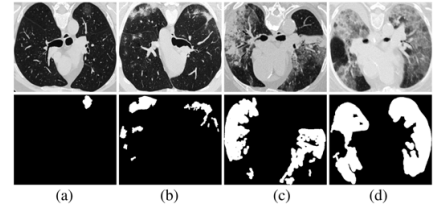
\includegraphics[width=\columnwidth,height=8cm]{sections/LBP/use1.png}
\captionof{figure}{Lung infection segmentation}
\vspace{0.5cm}
Concealed Object Detection can be used in the lung infection segmentation task in the medical field. Recently, COVID-19 has been of particular concern, and resulted in a global pandemic. An AI system equipped with a COVID-19 lung infection segmentation model would be helpful in the early screening of COVID-19.

\vspace{0.5cm}
\subsection{{{\fontsize{14}{19}\selectfont \textbf{Manufacturing}}}}
In industrial manufacturing, products (e.g., wood, textile, and magnetic tile) of poor quality will inevitably lead to adverse effects on the economy. The surface defects are challenging, with different factors including low contrast, ambiguous boundaries and so on. Since traditional surface defect detection systems mainly rely on humans, major issues are highly subjective and time-consuming to identify.
Thus, designing an automatic recognition system based on AI is essential to increase productivity.

\vspace{0.5cm}
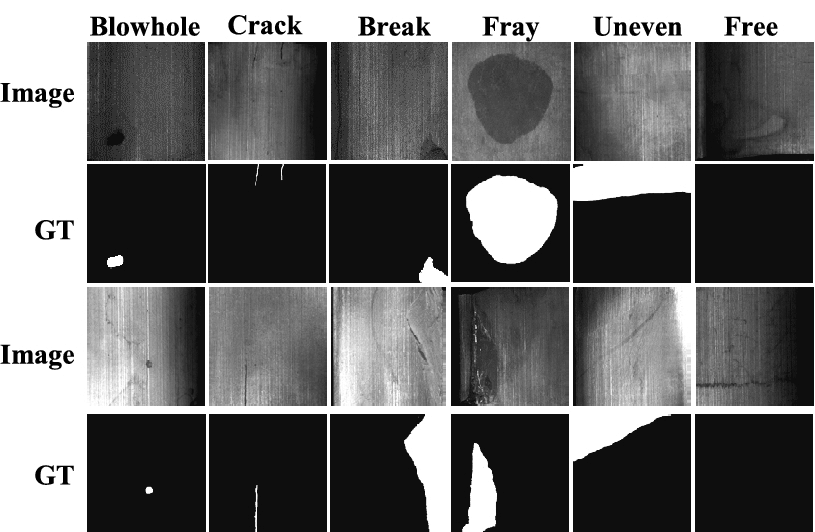
\includegraphics[width=\columnwidth,height=8cm]{sections/LBP/Examples-of-https-githubcom-abin24-Magnetic-tile-defect-datasets-magnetic-tile-surface.png}
\captionof{figure}{Surface Defect Detection}
\vspace{0.5cm}
\subsection{{{\fontsize{14}{19}\selectfont \textbf{Agriculture}}}}
\vspace{0.5cm}
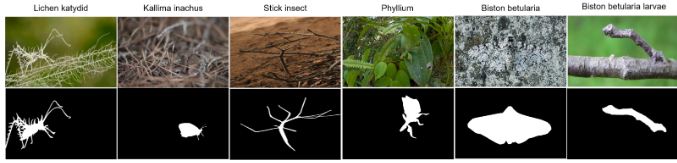
\includegraphics[width=\columnwidth,height=8cm]{sections/LBP/use2.png}
\captionof{figure}{Pest Detection}
\vspace{0.5cm}
Since the beginning of 2020, desert locust plagues have spread across multiple regions of the world, including Africa and South Asia. These swarms of locusts have caused significant damage to fields and crops, resulting in substantial economic losses and creating the potential for famine due to food shortages. To address this issue, governments could implement AI-based monitoring techniques, which would offer a more sustainable means of controlling the locust populations. However, obtaining relevant insect data for the development of accurate models is a significant challenge that requires a thorough understanding of insect biology.

\vspace{0.5cm}
\subsection{{{\fontsize{14}{19}\selectfont \textbf{Art}}}}
\vspace{0.5cm}
Camouflage detection is a useful tool in the field of art that allows experts to gain a deeper understanding of artwork. In the case of historical art, camouflaged elements may have been intentionally hidden by artists to convey hidden messages or symbols. By using specialized techniques such as infrared reflectography, X-ray imaging, or ultraviolet light, art historians and conservators can uncover these hidden elements and gain a deeper understanding of the artwork and the artist's intentions.

\vspace{0.5cm}
\subsection{{{\fontsize{14}{19}\selectfont \textbf{Military}}}}
\vspace{0.5cm}
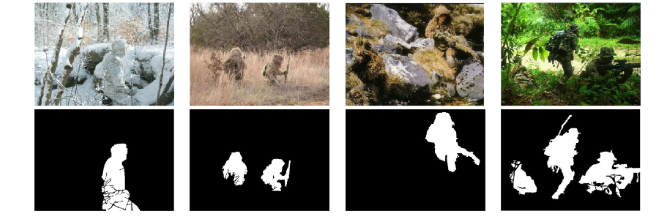
\includegraphics[width=\columnwidth,height=8cm]{sections/LBP/use3.png}
\captionof{figure}{Camouflaged military personnels in different environments}
\vspace{0.5cm}
Camouflage detection models can be extremely useful in military operations as they can help to identify enemy targets that may be hidden or difficult to spot using traditional visual methods. These models use advanced algorithms and machine learning techniques to analyze images and identify patterns that may indicate the presence of camouflage.\\
One of the primary uses of camouflage detection models in the military is for reconnaissance and surveillance missions. By analyzing satellite or drone images, these models can identify hidden enemy positions, camouflage nets, and other structures that may be used to conceal military equipment or personnel. This information can then be used to plan strategic strikes or to develop countermeasures to neutralize the enemy's camouflage.\\
Camouflage detection models can also be used to enhance the effectiveness of soldiers on the ground. For example, a soldier equipped with a helmet-mounted camera and a portable device that runs a real-time camouflage detection model could quickly identify hidden threats and provide valuable information to his or her squad.

\vspace{0.5cm}
\subsection{{{\fontsize{14}{19}\selectfont \textbf{Daily Life}}}}
\vspace{0.5cm}
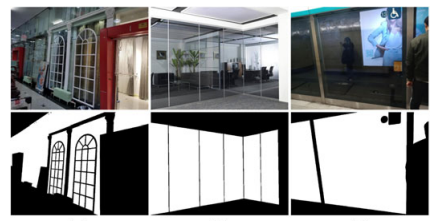
\includegraphics[width=\columnwidth,height=8cm]{sections/LBP/use4.png}
\captionof{figure}{Pest Detection}
\vspace{0.5cm}
Transparent objects, such as glass products, are commonplace in our daily life. These objects/things, including doors and walls, inherit the appearance of their background, making them unnoticeable. As a sub-task of COD, transparent object detection  and transparent object tracking have shown promise.
\end{multicols}

\vspace{0.5cm}
{\color{gray}\hrule}
\vspace{0.5cm}
